\documentclass{ximera}

%\usepackage{todonotes}

\newcommand{\todo}{}

\usepackage{esint} % for \oiint
\ifxake%%https://math.meta.stackexchange.com/questions/9973/how-do-you-render-a-closed-surface-double-integral
\renewcommand{\oiint}{{\large\bigcirc}\kern-1.56em\iint}
\fi


\graphicspath{
  {./}
  {ximeraTutorial/}
  {basicPhilosophy/}
  {functionsOfSeveralVariables/}
  {normalVectors/}
  {lagrangeMultipliers/}
  {vectorFields/}
  {greensTheorem/}
  {shapeOfThingsToCome/}
  {dotProducts/}
  {partialDerivativesAndTheGradientVector/}
  {../productAndQuotientRules/exercises/}
  {../normalVectors/exercisesParametricPlots/}
  {../continuityOfFunctionsOfSeveralVariables/exercises/}
  {../partialDerivativesAndTheGradientVector/exercises/}
  {../directionalDerivativeAndChainRule/exercises/}
  {../commonCoordinates/exercisesCylindricalCoordinates/}
  {../commonCoordinates/exercisesSphericalCoordinates/}
  {../greensTheorem/exercisesCurlAndLineIntegrals/}
  {../greensTheorem/exercisesDivergenceAndLineIntegrals/}
  {../shapeOfThingsToCome/exercisesDivergenceTheorem/}
  {../greensTheorem/}
  {../shapeOfThingsToCome/}
  {../separableDifferentialEquations/exercises/}
  {vectorFields/}
}

\newcommand{\mooculus}{\textsf{\textbf{MOOC}\textnormal{\textsf{ULUS}}}}

\usepackage{tkz-euclide}
\usepackage{tikz}
\usepackage{tikz-cd}
\usetikzlibrary{arrows}
\tikzset{>=stealth,commutative diagrams/.cd,
  arrow style=tikz,diagrams={>=stealth}} %% cool arrow head
\tikzset{shorten <>/.style={ shorten >=#1, shorten <=#1 } } %% allows shorter vectors

\usetikzlibrary{backgrounds} %% for boxes around graphs
\usetikzlibrary{shapes,positioning}  %% Clouds and stars
\usetikzlibrary{matrix} %% for matrix
\usepgfplotslibrary{polar} %% for polar plots
\usepgfplotslibrary{fillbetween} %% to shade area between curves in TikZ
%\usetkzobj{all}
\usepackage[makeroom]{cancel} %% for strike outs
%\usepackage{mathtools} %% for pretty underbrace % Breaks Ximera
%\usepackage{multicol}
\usepackage{pgffor} %% required for integral for loops



%% http://tex.stackexchange.com/questions/66490/drawing-a-tikz-arc-specifying-the-center
%% Draws beach ball
\tikzset{pics/carc/.style args={#1:#2:#3}{code={\draw[pic actions] (#1:#3) arc(#1:#2:#3);}}}



\usepackage{array}
\setlength{\extrarowheight}{+.1cm}
\newdimen\digitwidth
\settowidth\digitwidth{9}
\def\divrule#1#2{
\noalign{\moveright#1\digitwidth
\vbox{\hrule width#2\digitwidth}}}




% \newcommand{\RR}{\mathbb R}
% \newcommand{\R}{\mathbb R}
% \newcommand{\N}{\mathbb N}
% \newcommand{\Z}{\mathbb Z}

\newcommand{\sagemath}{\textsf{SageMath}}


%\renewcommand{\d}{\,d\!}
%\renewcommand{\d}{\mathop{}\!d}
%\newcommand{\dd}[2][]{\frac{\d #1}{\d #2}}
%\newcommand{\pp}[2][]{\frac{\partial #1}{\partial #2}}
% \renewcommand{\l}{\ell}
%\newcommand{\ddx}{\frac{d}{\d x}}

% \newcommand{\zeroOverZero}{\ensuremath{\boldsymbol{\tfrac{0}{0}}}}
%\newcommand{\inftyOverInfty}{\ensuremath{\boldsymbol{\tfrac{\infty}{\infty}}}}
%\newcommand{\zeroOverInfty}{\ensuremath{\boldsymbol{\tfrac{0}{\infty}}}}
%\newcommand{\zeroTimesInfty}{\ensuremath{\small\boldsymbol{0\cdot \infty}}}
%\newcommand{\inftyMinusInfty}{\ensuremath{\small\boldsymbol{\infty - \infty}}}
%\newcommand{\oneToInfty}{\ensuremath{\boldsymbol{1^\infty}}}
%\newcommand{\zeroToZero}{\ensuremath{\boldsymbol{0^0}}}
%\newcommand{\inftyToZero}{\ensuremath{\boldsymbol{\infty^0}}}



% \newcommand{\numOverZero}{\ensuremath{\boldsymbol{\tfrac{\#}{0}}}}
% \newcommand{\dfn}{\textbf}
% \newcommand{\unit}{\,\mathrm}
% \newcommand{\unit}{\mathop{}\!\mathrm}
% \newcommand{\eval}[1]{\bigg[ #1 \bigg]}
% \newcommand{\seq}[1]{\left( #1 \right)}
% \renewcommand{\epsilon}{\varepsilon}
% \renewcommand{\phi}{\varphi}


% \renewcommand{\iff}{\Leftrightarrow}

% \DeclareMathOperator{\arccot}{arccot}
% \DeclareMathOperator{\arcsec}{arcsec}
% \DeclareMathOperator{\arccsc}{arccsc}
% \DeclareMathOperator{\si}{Si}
% \DeclareMathOperator{\scal}{scal}
% \DeclareMathOperator{\sign}{sign}


%% \newcommand{\tightoverset}[2]{% for arrow vec
%%   \mathop{#2}\limits^{\vbox to -.5ex{\kern-0.75ex\hbox{$#1$}\vss}}}
% \newcommand{\arrowvec}[1]{{\overset{\rightharpoonup}{#1}}}
% \renewcommand{\vec}[1]{\arrowvec{\mathbf{#1}}}
% \renewcommand{\vec}[1]{{\overset{\boldsymbol{\rightharpoonup}}{\mathbf{#1}}}}

% \newcommand{\point}[1]{\left(#1\right)} %this allows \vector{ to be changed to \vector{ with a quick find and replace
% \newcommand{\pt}[1]{\mathbf{#1}} %this allows \vec{ to be changed to \vec{ with a quick find and replace
% \newcommand{\Lim}[2]{\lim_{\point{#1} \to \point{#2}}} %Bart, I changed this to point since I want to use it.  It runs through both of the exercise and exerciseE files in limits section, which is why it was in each document to start with.

% \DeclareMathOperator{\proj}{\mathbf{proj}}
% \newcommand{\veci}{{\boldsymbol{\hat{\imath}}}}
% \newcommand{\vecj}{{\boldsymbol{\hat{\jmath}}}}
% \newcommand{\veck}{{\boldsymbol{\hat{k}}}}
% \newcommand{\vecl}{\vec{\boldsymbol{\l}}}
% \newcommand{\uvec}[1]{\mathbf{\hat{#1}}}
% \newcommand{\utan}{\mathbf{\hat{t}}}
% \newcommand{\unormal}{\mathbf{\hat{n}}}
% \newcommand{\ubinormal}{\mathbf{\hat{b}}}

% \newcommand{\dotp}{\bullet}
% \newcommand{\cross}{\boldsymbol\times}
% \newcommand{\grad}{\boldsymbol\nabla}
% \newcommand{\divergence}{\grad\dotp}
% \newcommand{\curl}{\grad\cross}
%\DeclareMathOperator{\divergence}{divergence}
%\DeclareMathOperator{\curl}[1]{\grad\cross #1}
% \newcommand{\lto}{\mathop{\longrightarrow\,}\limits}

% \renewcommand{\bar}{\overline}

\colorlet{textColor}{black}
\colorlet{background}{white}
\colorlet{penColor}{blue!50!black} % Color of a curve in a plot
\colorlet{penColor2}{red!50!black}% Color of a curve in a plot
\colorlet{penColor3}{red!50!blue} % Color of a curve in a plot
\colorlet{penColor4}{green!50!black} % Color of a curve in a plot
\colorlet{penColor5}{orange!80!black} % Color of a curve in a plot
\colorlet{penColor6}{yellow!70!black} % Color of a curve in a plot
\colorlet{fill1}{penColor!20} % Color of fill in a plot
\colorlet{fill2}{penColor2!20} % Color of fill in a plot
\colorlet{fillp}{fill1} % Color of positive area
\colorlet{filln}{penColor2!20} % Color of negative area
\colorlet{fill3}{penColor3!20} % Fill
\colorlet{fill4}{penColor4!20} % Fill
\colorlet{fill5}{penColor5!20} % Fill
\colorlet{gridColor}{gray!50} % Color of grid in a plot

\newcommand{\surfaceColor}{violet}
\newcommand{\surfaceColorTwo}{redyellow}
\newcommand{\sliceColor}{greenyellow}




\pgfmathdeclarefunction{gauss}{2}{% gives gaussian
  \pgfmathparse{1/(#2*sqrt(2*pi))*exp(-((x-#1)^2)/(2*#2^2))}%
}


%%%%%%%%%%%%%
%% Vectors
%%%%%%%%%%%%%

%% Simple horiz vectors
\renewcommand{\vector}[1]{\left\langle #1\right\rangle}


%% %% Complex Horiz Vectors with angle brackets
%% \makeatletter
%% \renewcommand{\vector}[2][ , ]{\left\langle%
%%   \def\nextitem{\def\nextitem{#1}}%
%%   \@for \el:=#2\do{\nextitem\el}\right\rangle%
%% }
%% \makeatother

%% %% Vertical Vectors
%% \def\vector#1{\begin{bmatrix}\vecListA#1,,\end{bmatrix}}
%% \def\vecListA#1,{\if,#1,\else #1\cr \expandafter \vecListA \fi}

%%%%%%%%%%%%%
%% End of vectors
%%%%%%%%%%%%%

%\newcommand{\fullwidth}{}
%\newcommand{\normalwidth}{}



%% makes a snazzy t-chart for evaluating functions
%\newenvironment{tchart}{\rowcolors{2}{}{background!90!textColor}\array}{\endarray}

%%This is to help with formatting on future title pages.
\newenvironment{sectionOutcomes}{}{}



%% Flowchart stuff
%\tikzstyle{startstop} = [rectangle, rounded corners, minimum width=3cm, minimum height=1cm,text centered, draw=black]
%\tikzstyle{question} = [rectangle, minimum width=3cm, minimum height=1cm, text centered, draw=black]
%\tikzstyle{decision} = [trapezium, trapezium left angle=70, trapezium right angle=110, minimum width=3cm, minimum height=1cm, text centered, draw=black]
%\tikzstyle{question} = [rectangle, rounded corners, minimum width=3cm, minimum height=1cm,text centered, draw=black]
%\tikzstyle{process} = [rectangle, minimum width=3cm, minimum height=1cm, text centered, draw=black]
%\tikzstyle{decision} = [trapezium, trapezium left angle=70, trapezium right angle=110, minimum width=3cm, minimum height=1cm, text centered, draw=black]


\title{Left and Right}

\begin{document}

\begin{abstract}
sliding the graph
\end{abstract}
\maketitle






$\blacktriangleright$ Graphically, shifting the domain of a function appears to shift the graph horizontally - left or right.  The shape of the graph doesn't change.  The whole graph moves rigidly left or right.  All points move the same distance horizontally. \\


\begin{itemize}
\item Let $F(x)$ be a function with its domain.

\item Let $G(t)$ be a new function defined as $G(t) = F(t+d_0)$ with its induced domain, where $d_0$ is a fixed constant.
\end{itemize}



We begin with the function $F$.  The domain values of $F$ are represented by $x$.  We then define a new function, $G$. The domain values of $G$ are represented by $t$. 

$F$ and $G$ are connected.  To evaluate $G$ at $t$, you evaluate $F$ at $t + d_0$, where $d_0$ is some constant.  Therefore, $t + d_0$ are $x$-values. We have $x = t + d_0$.  This tells us what to do to $t$ to get $x$.  However, that is not how our story is told.  Our story begins with $F$ and then $G$ is defined from $F$.  

We want to know how to get $t$ from $x$.  


\begin{itemize}
\item $x = t + d_0$

\item $x - d_0 = t$
\end{itemize}


To get corresponding values of $t$ from values of $x$, subtract $d_0$.   



$\blacktriangleright$  The graph of $G$ is obtained from the graph of $F$ by subtracting $d_0$ from domain values of $F$, which appears to be reverse of the definition, $G(t) = F(t+d_0)$.  That is because the definition tells how to get the old domain for $F$, rather than getting the new domain for $G$.



\begin{example} Shifting Horizontally




Graph of $y = T(v)$.

\begin{image}
\begin{tikzpicture}
	\begin{axis}[
            domain=-10:10, ymax=10, xmax=10, ymin=-10, xmin=-10,
            axis lines =center, xlabel=$v$, ylabel=$y$,
            ytick={-10,-8,-6,-4,-2,2,4,6,8,10},
            xtick={-10,-8,-6,-4,-2,2,4,6,8,10},
            ticklabel style={font=\scriptsize},
            every axis y label/.style={at=(current axis.above origin),anchor=south},
            every axis x label/.style={at=(current axis.right of origin),anchor=west},
            axis on top
          ]
          
	\addplot [draw=penColor,very thick,smooth,domain=(-7:-4)] {-x-6};
	\addplot [draw=penColor,very thick,smooth,domain=(-2:1)] {-7};
	\addplot [draw=penColor,very thick,smooth,domain=(1:7)] {-x+7};
	
	\addplot[color=penColor,only marks,mark=*] coordinates{(-7,1)}; 
	\addplot[color=penColor,fill=white,only marks,mark=*] coordinates{(-4,-2)}; 
	\addplot[color=penColor,only marks,mark=*] coordinates{(-2,-7)}; 
	\addplot[color=penColor,only marks,mark=*] coordinates{(1,-7)}; 
	\addplot[color=penColor,only marks,mark=*] coordinates{(1,6)}; 
	\addplot[color=penColor,fill=white,only marks,mark=*] coordinates{(7,0)}; 


    \end{axis}
\end{tikzpicture}
\end{image}


Define a new function $W$ by $W(h)=T(h+3)$, with the induced domain.

Which graph below is the graph of $z=W(h)$?





\begin{image}
\begin{tikzpicture}
	\begin{axis}[name = leftgraph,
            domain=-10:10, ymax=10, xmax=10, ymin=-10, xmin=-10,
            axis lines =center, xlabel=$h$, ylabel=$z$,
            ytick={-10,-8,-6,-4,-2,2,4,6,8,10},
            xtick={-10,-8,-6,-4,-2,2,4,6,8,10},
            ticklabel style={font=\scriptsize},
            every axis y label/.style={at=(current axis.above origin),anchor=south},
            every axis x label/.style={at=(current axis.right of origin),anchor=west},
            axis on top
          ]
          
	\addplot [draw=penColor,very thick,smooth,domain=(-10:-7)] {-(x+3)-6};
	\addplot [draw=penColor,very thick,smooth,domain=(-5:-2)] {-7};
	\addplot [draw=penColor,very thick,smooth,domain=(-2:4)] {-(x+3)+7};
	
	\addplot[color=penColor,only marks,mark=*] coordinates{(-10,1)}; 
	\addplot[color=penColor,fill=white,only marks,mark=*] coordinates{(-7,-2)}; 
	\addplot[color=penColor,only marks,mark=*] coordinates{(-5,-7)}; 
	\addplot[color=penColor,only marks,mark=*] coordinates{(-2,-7)}; 
	\addplot[color=penColor,only marks,mark=*] coordinates{(-2,6)}; 
	\addplot[color=penColor,fill=white,only marks,mark=*] coordinates{(4,0)}; 


    \end{axis}
	\begin{axis}[at={(leftgraph.outer east)},anchor=outer west, 
            domain=-10:10, ymax=10, xmax=10, ymin=-10, xmin=-10,
            axis lines =center, xlabel=$h$, ylabel=$z$,
            ytick={-10,-8,-6,-4,-2,2,4,6,8,10},
            xtick={-10,-8,-6,-4,-2,2,4,6,8,10},
            ticklabel style={font=\scriptsize},
            every axis y label/.style={at=(current axis.above origin),anchor=south},
            every axis x label/.style={at=(current axis.right of origin),anchor=west},
            axis on top
          ]
          
	\addplot [draw=penColor,very thick,smooth,domain=(-4:-1)] {-(x-3)-6};
	\addplot [draw=penColor,very thick,smooth,domain=(1:4)] {-7};
	\addplot [draw=penColor,very thick,smooth,domain=(4:10)] {-(x-3)+7};
	
	\addplot[color=penColor,only marks,mark=*] coordinates{(-4,1)}; 
	\addplot[color=penColor,fill=white,only marks,mark=*] coordinates{(-1,-2)}; 
	\addplot[color=penColor,only marks,mark=*] coordinates{(1,-7)}; 
	\addplot[color=penColor,only marks,mark=*] coordinates{(4,-7)}; 
	\addplot[color=penColor,only marks,mark=*] coordinates{(4,6)}; 
	\addplot[color=penColor,fill=white,only marks,mark=*] coordinates{(10,0)}; 


    \end{axis}


\end{tikzpicture}
\end{image}





\begin{multipleChoice}
\choice[correct]{graph on the left}
\choice{graph on the right}
\end{multipleChoice}

To figure this out, we need to know how to get the new variable $h$ from the old variable $v$. \\




\begin{itemize}
\item $h$ represents the domain of $W$. 
\item $v$ represents the domain of $T$.  
\item $v$ = $h+3$
\end{itemize}


These tell us that $v-3 = h$ and the graph of $W$ is the graph of $T$ shifted left $3$.



\end{example}


The shape of the graph didn't change. It just slid to the left. There are still three pieces. \\




\begin{itemize}
\item The domain still has a gap of length $2$ in it.  
\item The middle piece is still horizontal.  
\item The solid and hollow endpoint dots are still in the same positions. 
\end{itemize}





Shifting doesn't change the shape of the graph or any of the relative measurements. It is a rigid movement.












\begin{example} Sine



Graph of $y = \sin(\theta)$.

\begin{image}
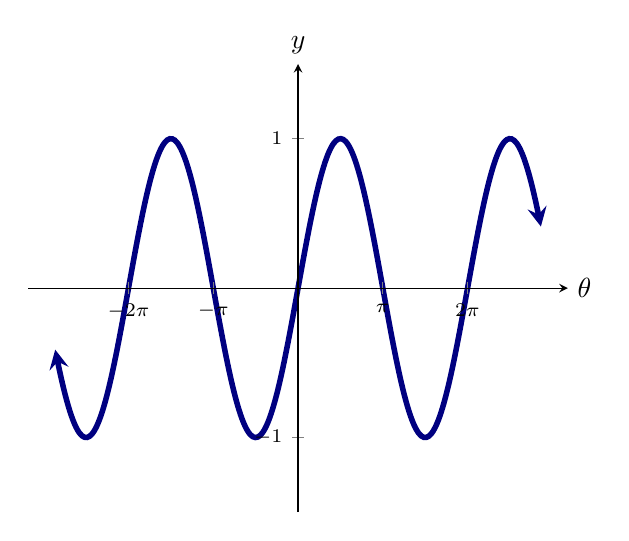
\begin{tikzpicture} 
  \begin{axis}[
            domain=-10:10, ymax=1.5, xmax=10, ymin=-1.5, xmin=-10,
            xtick={-6.28, -3.14, 3.14, 6.28}, 
            xticklabels={$-2\pi$, $-\pi$, $\pi$, $2\pi$},
            axis lines =center,  xlabel={$\theta$}, ylabel=$y$,
            ticklabel style={font=\scriptsize},
            every axis y label/.style={at=(current axis.above origin),anchor=south},
            every axis x label/.style={at=(current axis.right of origin),anchor=west},
            axis on top
          ]
          
            \addplot [line width=2, penColor, smooth,samples=200,domain=(-9:9), <->] {sin(deg(x))};

           

  \end{axis}
\end{tikzpicture}
\end{image}



Let's create a new function called $T$, which is a shifted sine function.

\[  T(t) = \sin(t + \tfrac{\pi}{6})  \]



\begin{image}
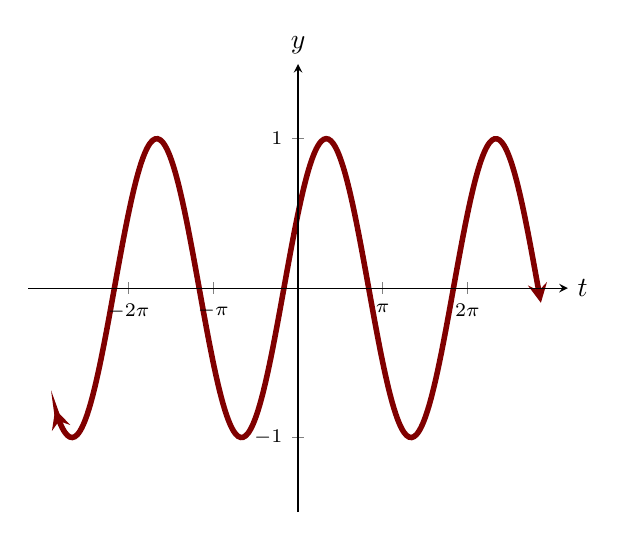
\begin{tikzpicture} 
  \begin{axis}[
            domain=-10:10, ymax=1.5, xmax=10, ymin=-1.5, xmin=-10,
            xtick={-6.28, -3.14, 3.14, 6.28}, 
            xticklabels={$-2\pi$, $-\pi$, $\pi$, $2\pi$},
            axis lines =center,  xlabel={$t$}, ylabel=$y$,
            ticklabel style={font=\scriptsize},
            every axis y label/.style={at=(current axis.above origin),anchor=south},
            every axis x label/.style={at=(current axis.right of origin),anchor=west},
            axis on top
          ]
          
            \addplot [line width=2, penColor2, smooth,samples=200,domain=(-9:9), <->] {sin(deg(x+0.523599))};

           

  \end{axis}
\end{tikzpicture}
\end{image}
This graph looks the same as the one above, except shifted to the left.


$\theta = t + \tfrac{\pi}{6}$   or $\theta - \tfrac{\pi}{6}= t $



Labelling the horizontal axes $\theta$ and $t$ makes it easier to compare.

\end{example}









\begin{image}
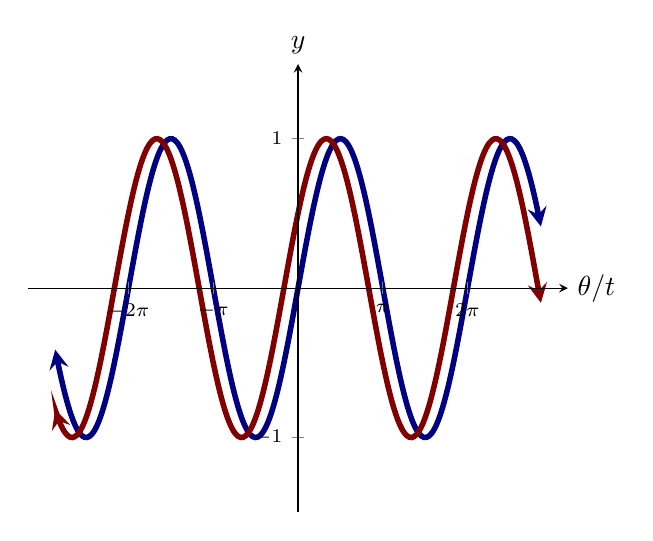
\begin{tikzpicture} 
  \begin{axis}[
            domain=-10:10, ymax=1.5, xmax=10, ymin=-1.5, xmin=-10,
            xtick={-6.28, -3.14, 3.14, 6.28}, 
            xticklabels={$-2\pi$, $-\pi$, $\pi$, $2\pi$},
            axis lines =center,  xlabel={$\theta$/$t$}, ylabel=$y$,
            ticklabel style={font=\scriptsize},
            every axis y label/.style={at=(current axis.above origin),anchor=south},
            every axis x label/.style={at=(current axis.right of origin),anchor=west},
            axis on top
          ]
          
            \addplot [line width=2, penColor, smooth,samples=200,domain=(-9:9), <->] {sin(deg(x))};
            \addplot [line width=2, penColor2, smooth,samples=200,domain=(-9:9), <->] {sin(deg(x+0.523599))};

           

  \end{axis}
\end{tikzpicture}
\end{image}











\begin{example} Sine



Graph of $y = \sin(\theta)$.

\begin{image}
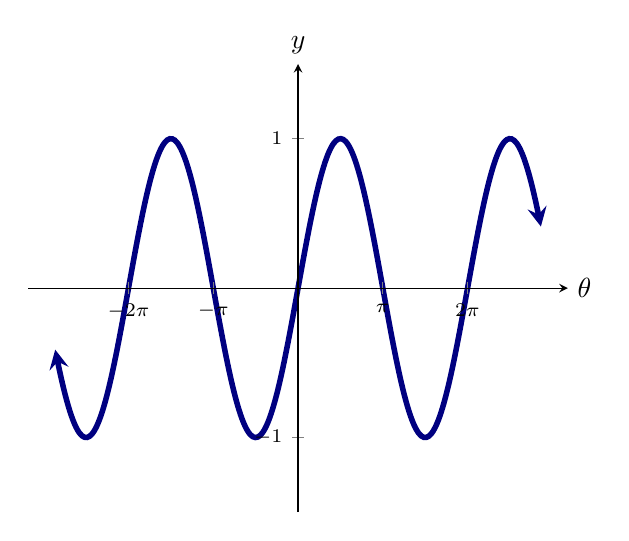
\begin{tikzpicture} 
  \begin{axis}[
            domain=-10:10, ymax=1.5, xmax=10, ymin=-1.5, xmin=-10,
            xtick={-6.28, -3.14, 3.14, 6.28}, 
            xticklabels={$-2\pi$, $-\pi$, $\pi$, $2\pi$},
            axis lines =center,  xlabel={$\theta$}, ylabel=$y$,
            ticklabel style={font=\scriptsize},
            every axis y label/.style={at=(current axis.above origin),anchor=south},
            every axis x label/.style={at=(current axis.right of origin),anchor=west},
            axis on top
          ]
          
          	\addplot [line width=2, penColor, smooth,samples=200,domain=(-9:9), <->] {sin(deg(x))};

           

  \end{axis}
\end{tikzpicture}
\end{image}



$\sin(\theta)$ is periodic with a period of $2\pi$.  If it is shifted by $2\pi$ or any integer multiple of $2\pi$, then the resulting function is again $\sin(\theta)$.


\[    \sin(\theta + 2k\pi) = \sin(\theta)   \,   \text{ where }  \,  k \in \textbf{Z}       \]



\begin{itemize}
\item The zeros of $\sin(\theta)$ are all integer multiples of $\pi$.
\item The maximum value is $1$ and it occurs at:  $\left\{     \frac{\pi}{2} + 2k\pi \, | \, k \in \textbf{Z}     \right\} = \left\{     \frac{(4k+1)\pi}{2} \, | \, k \in \textbf{Z}     \right\}$
\item The minimum value is $-1$ and it occurs at:  $\left\{    \frac{3\pi}{2} + 2k\pi \, | \, k \in \textbf{Z}     \right\} = \left\{    \frac{(4k+3)\pi}{2} \, | \, k \in \textbf{Z}     \right\}$
\end{itemize}


If $\sin(\theta)$ is shifted left by $\frac{\pi}{2}$, then we get $\cos(\theta)$.


\[    \sin\left(\theta + \frac{\pi}{2}\right) = \cos(\theta)   \]


Graph of $y = \cos(\theta)$.

\begin{image}
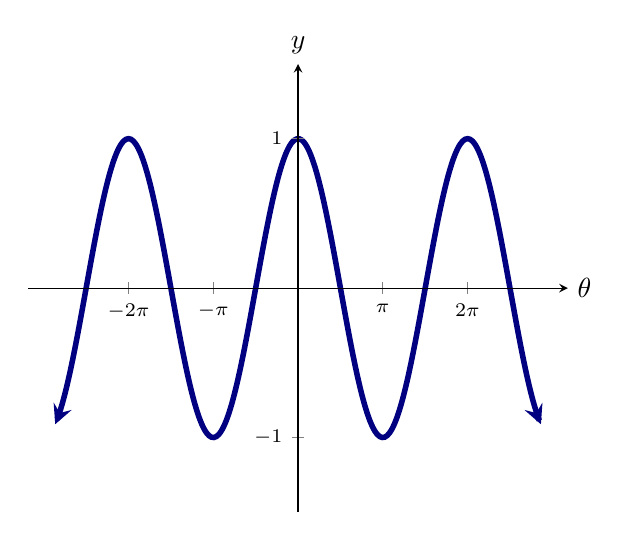
\begin{tikzpicture} 
  \begin{axis}[
            domain=-10:10, ymax=1.5, xmax=10, ymin=-1.5, xmin=-10,
            xtick={-6.28, -3.14, 3.14, 6.28}, 
            xticklabels={$-2\pi$, $-\pi$, $\pi$, $2\pi$},
            axis lines =center,  xlabel={$\theta$}, ylabel=$y$,
            ticklabel style={font=\scriptsize},
            every axis y label/.style={at=(current axis.above origin),anchor=south},
            every axis x label/.style={at=(current axis.right of origin),anchor=west},
            axis on top
          ]
          
          	\addplot [line width=2, penColor, smooth,samples=200,domain=(-9:9), <->] {cos(deg(x))};

           

  \end{axis}
\end{tikzpicture}
\end{image}



\end{example}




This agrees with the unit circle.  As you move along the unit circle, the right/vertical coordinate (sine) has the same value as the left/horizontal coordinate (cosine) back a quarter-circle.









\begin{example} Absolute Value



Graph of $y = |x|$.



\begin{image}
\begin{tikzpicture} 
  \begin{axis}[
            domain=-10:10, ymax=10, xmax=10, ymin=-10, xmin=-10,
            axis lines =center, xlabel=$x$, ylabel=$y$,
            ytick={-10,-8,-6,-4,-2,2,4,6,8,10},
            xtick={-10,-8,-6,-4,-2,2,4,6,8,10},
            ticklabel style={font=\scriptsize},
            every axis y label/.style={at=(current axis.above origin),anchor=south},
            every axis x label/.style={at=(current axis.right of origin),anchor=west},
            axis on top
          ]
          
          \addplot [line width=2, penColor, smooth, samples=200, domain=(-7:7),<->] {abs(x)};
        

  \end{axis}
\end{tikzpicture}
\end{image}





What does the graph of $z = |t-2|$ look like?

This is a shift from the basic absolute value graph.  All we really need to know is where is the corner.  

\begin{center}
\textbf{\textcolor{blue!55!black}{The corner occurs when the inside of the absolute value equals $0$.}} 
\end{center}



$t-2=0$ when $t=2$.  That is where the new corner sits.









\begin{image}
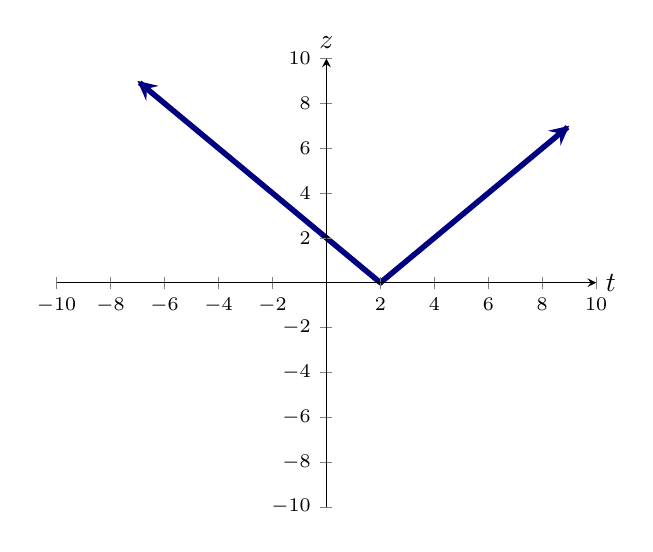
\begin{tikzpicture} 
  \begin{axis}[
            domain=-10:10, ymax=10, xmax=10, ymin=-10, xmin=-10,
            axis lines =center, xlabel=$t$, ylabel=$z$,
            ytick={-10,-8,-6,-4,-2,2,4,6,8,10},
            xtick={-10,-8,-6,-4,-2,2,4,6,8,10},
            ticklabel style={font=\scriptsize},
            every axis y label/.style={at=(current axis.above origin),anchor=south},
            every axis x label/.style={at=(current axis.right of origin),anchor=west},
            axis on top
          ]
          
          \addplot [line width=2, penColor, smooth, samples=200, domain=(-7:9),<->] {abs(x-2)};
        

  \end{axis}
\end{tikzpicture}
\end{image}








\end{example}


Much of graphing follows this example.  \\


There are \textbf{important/strategic points} for the function's graph. You identify the new position of those points.  Then, the shifted graph follows the basic shape of the original graph.






For example, $y = \log_k(t)$ [ including $y = \ln(t)$ ] has a vertical asymptote when the inside of the logarithm equals $0$. The zero, and corresponding horizontal intercept, occurs when the inside equals $1$.  






\begin{example}

Here is the graph of $y = \log_2(t+5)$.

\begin{itemize}
\item vertical asymptote: $t+5=0$, when $t=\answer{-5}$
\item horizontal intercept: $t+5=1$, when $t=\answer{-4}$
\end{itemize}


\begin{image}
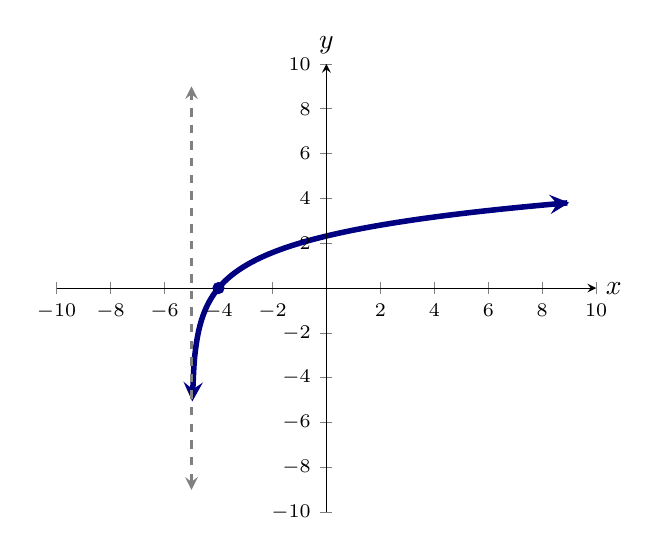
\begin{tikzpicture} 
  \begin{axis}[
            domain=-10:10, ymax=10, xmax=10, ymin=-10, xmin=-10,
            axis lines =center, xlabel=$x$, ylabel=$y$,
            ytick={-10,-8,-6,-4,-2,2,4,6,8,10},
            xtick={-10,-8,-6,-4,-2,2,4,6,8,10},
            ticklabel style={font=\scriptsize},
            every axis y label/.style={at=(current axis.above origin),anchor=south},
            every axis x label/.style={at=(current axis.right of origin),anchor=west},
            axis on top
          ]
          
          \addplot [line width=2, penColor, smooth,samples=200,domain=(-4.97:9),<->] {ln(x+5)/ln(2)};
          \addplot [line width=1, gray, dashed,domain=(-9:9),<->] ({-5},{x});

          \addplot[color=penColor,only marks,mark=*] coordinates{(-4,0)}; 

           

  \end{axis}
\end{tikzpicture}
\end{image}


The graph looks the same as the basic logarithm graph, just slid left $5$.




\end{example}









\begin{example} Shifting Domains


Let $M$ be a function with domain $[-7,-4) \cup [-2,1] \cup [1,7)$. \\

Below is the graph of $y = M(d)$.




\begin{image}
\begin{tikzpicture}
  \begin{axis}[
            domain=-10:10, ymax=10, xmax=10, ymin=-10, xmin=-10,
            axis lines =center, xlabel=$d$, ylabel=$y$,
            ytick={-10,-8,-6,-4,-2,2,4,6,8,10},
            xtick={-10,-8,-6,-4,-2,2,4,6,8,10},
            ticklabel style={font=\scriptsize},
            every axis y label/.style={at=(current axis.above origin),anchor=south},
            every axis x label/.style={at=(current axis.right of origin),anchor=west},
            axis on top
          ]
          
  \addplot [draw=penColor,very thick,smooth,domain=(-7:-4)] {-x-6};
  \addplot [draw=penColor,very thick,smooth,domain=(-2:1)] {-7};
  \addplot [draw=penColor,very thick,smooth,domain=(1:7)] {-x+7};
  
  \addplot[color=penColor,only marks,mark=*] coordinates{(-7,1)}; 
  \addplot[color=penColor,fill=white,only marks,mark=*] coordinates{(-4,-2)}; 
  \addplot[color=penColor,only marks,mark=*] coordinates{(-2,-7)}; 
  \addplot[color=penColor,only marks,mark=*] coordinates{(1,-7)}; 
  \addplot[color=penColor,only marks,mark=*] coordinates{(1,6)}; 
  \addplot[color=penColor,fill=white,only marks,mark=*] coordinates{(7,0)}; 


    \end{axis}
\end{tikzpicture}
\end{image}
A new function is created by shifting $M$. \\





The function $H(k)$ is defined as $H(k) = M(k+3)$ with the induced domain.



\begin{question}

We can see that $M(-7) = 1$.  This tells us that $H\left(\answer{-10}\right) = \answer{1}$. \\

There is an open dot on the graph of $y= M(d)$  when $d = -4$.  There will be a corresponding open dot on the graph of $z = H(k)$ when $k = \answer{-7}$.

\end{question}


\begin{question}

There is a horizontal line segment in the graph of $y = M(d)$ from $(-2, -7)$ to $(1, -7)$.  There will be a horizontal line segment in the graph of $z = H(k)$ from $\left(\answer{-5}, -7\right)$ to $\left(\answer{-2}, -7\right)$.

\end{question}



\begin{question}

There is a closed dot on the graph of $y= M(d)$  when $d = 1$.  There will be a corresponding closed dot on the graph of $z = H(k)$ when $k = \answer{-2}$. \\


There is an open dot on the graph of $y= M(d)$  when $d = 7$.  There will be a corresponding open dot on the graph of $z = H(k)$ when $k = \answer{4}$.

\end{question}




\end{example}


























\begin{center}
\textbf{\textcolor{green!50!black}{oooo-=-=-=-ooOoo-=-=-=-ooooo}} \\

more examples can be found by following this link\\ \link[More Examples of Shifting]{https://ximera.osu.edu/csccmathematics/precalculus1/precalculus1/shifting/examples/exampleList}

\end{center}






\end{document}
